Results go here. Refer to figures, tables, equations and other sections with
\texttt{cleveref}, e.g.\ \cref{sec:methods} describes the procedure, \cref{fig:example}
shows the response, \cref{tab:example} summarizes the parameters, and the model is given
by \cref{eq:example}.

% --- Example equation block -------------------------------------------------
The membrane potential $V$ evolves according to a leaky integrator,
\begin{equation}\label{eq:example}
  \tau \frac{\mathrm{d}V}{\mathrm{d}t} = -\bigl(V - V_{\mathrm{rest}}\bigr) + R\,I(t),
\end{equation}
with membrane time constant $\tau$, resting potential $V_{\mathrm{rest}}$, input
resistance $R$, and input current $I(t)$. For an unnumbered display, use
\verb|\[ ... \]| or the \texttt{equation*} environment.

% --- Example figure with caption --------------------------------------------
\begin{figure}[htbp]
  \centering
  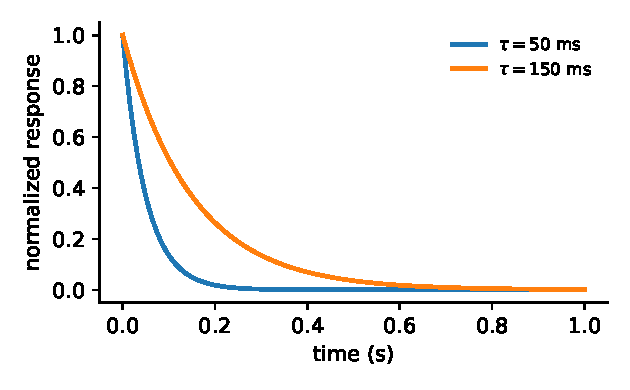
\includegraphics[width=0.6\linewidth]{figures/example-figure}
  \caption{\textbf{Example figure.} Normalized response of \cref{eq:example} to a step
    input for two membrane time constants. Replace \texttt{figures/example-figure.pdf}
    with your own (regenerate via \texttt{scripts/make-example-figure.py}). Captions use
    the \texttt{caption} package at \texttt{small} font.}
  \label{fig:example}
\end{figure}

% --- Example table with caption ---------------------------------------------
\begin{table}[htbp]
  \centering
  \caption{\textbf{Example parameters.} A \texttt{booktabs} table; its caption also uses
    the \texttt{caption} package at \texttt{small} font. Table captions go \emph{above}
    the tabular by convention.}
  \label{tab:example}
  \begin{tabular}{lcc}
    \toprule
    Parameter & Symbol & Value \\
    \midrule
    Membrane time constant & $\tau$              & $20$ ms \\
    Resting potential      & $V_{\mathrm{rest}}$ & $-65$ mV \\
    Input resistance       & $R$                 & $100$ M$\Omega$ \\
    \bottomrule
  \end{tabular}
\end{table}
